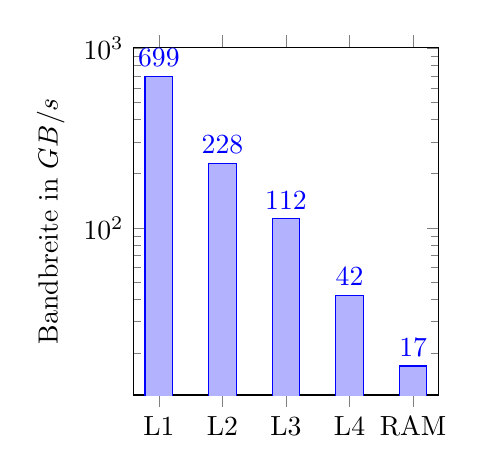
\begin{tikzpicture}
	\begin{axis}[
			height=6cm,
			width=0.45\textwidth,
			ybar,
			ymode=log,
			%extra tick style={grid=major},
			ylabel={Bandbreite in $GB/s$},
			symbolic x coords={L1, L2, L3, L4, RAM},
			xtick=data,
			nodes near coords,
			nodes near coords align={vertical}
		]
		\addplot+[point meta=explicit symbolic] 
		coordinates {
			(L1, 699) [699]
			(L2, 228) [228]
			(L3, 112) [112]
			(L4, 42) [42]
			(RAM, 17) [17]
		};
	\end{axis}
\end{tikzpicture}
